%%%%%%%% ICML 2025 EXAMPLE LATEX SUBMISSION FILE %%%%%%%%%%%%%%%%%

\documentclass{article}
% Recommended, but optional, packages for figures and better typesetting:
\usepackage{microtype}
\usepackage{graphicx}
\usepackage{subfigure}
\usepackage{booktabs} % for professional tables
\usepackage{subcaption}
\usepackage{caption}
\usepackage[all]{nowidow} % apparently helpful for keeping 2 column text in place and improves flow

% hyperref makes hyperlinks in the resulting PDF.
% If your build breaks (sometimes temporarily if a hyperlink spans a page)
% please comment out the following usepackage line and replace
% \usepackage{icml2025} with \usepackage[nohyperref]{icml2025} above.

\usepackage[hyphens]{url}
\usepackage{hyperref}


% Attempt to make hyperref and algorithmic work together better:
\newcommand{\theHalgorithm}{\arabic{algorithm}}

% Use the following line for the initial blind version submitted for review:
% \usepackage{icml2025}

% If accepted, instead use the following line for the camera-ready submission:
\usepackage[accepted]{icml2025}
\makeatletter
\renewcommand{\ICML@appearing}{}
\makeatother

% For theorems and such
\usepackage{amsmath}
\usepackage{amssymb}
\usepackage{mathtools}
\usepackage{amsthm}

% For tables
\usepackage{makecell}
\usepackage{booktabs}

% if you use cleveref..
\usepackage[capitalize,noabbrev]{cleveref}
\usepackage{xcolor}
\usepackage[normalem]{ulem} % for striking/crossing out text


\newcommand{\sw}[1]{\textcolor{blue}{SW: #1}}
\newcommand{\dl}[1]{\textcolor{violet}{DL: #1}}
\newcommand{\pulkit}[1]{\textcolor{orange}{PA: #1}}
\newcommand{\akarsh}[1]{\textcolor{red}{AK: #1}}
\newcommand{\akout}[1]{\textcolor{red}{\sout{#1}}}
\newcommand{\ryan}[1]{\textcolor{magenta}{RB: #1}}
\newcommand{\zs}[1]{\textcolor{green}{ZS: #1}}

% Newline
\newcommand{\pmnl}[2]{%
  $\begin{aligned}[t]#1\\[-1pt]\pm\,#2\end{aligned}$%
}

%%%%%%%%%%%%%%%%%%%%%%%%%%%%%%%%
% THEOREMS
%%%%%%%%%%%%%%%%%%%%%%%%%%%%%%%%
\theoremstyle{plain}
\newtheorem{theorem}{Theorem}[section]
\newtheorem{proposition}[theorem]{Proposition}
\newtheorem{lemma}[theorem]{Lemma}
\newtheorem{corollary}[theorem]{Corollary}
\theoremstyle{definition}
\newtheorem{definition}[theorem]{Definition}
\newtheorem{assumption}[theorem]{Assumption}
\theoremstyle{remark}
\newtheorem{remark}[theorem]{Remark}

% Todonotes is useful during development; simply uncomment the next line
%    and comment out the line below the next line to turn off comments
%\usepackage[disable,textsize=tiny]{todonotes}
\usepackage[textsize=tiny]{todonotes}


% The \icmltitle you define below is probably too long as a header.
% Therefore, a short form for the running title is supplied here:
\icmltitlerunning{Training Language Models via Neural Cellular Automata}

\begin{document}

\twocolumn[
\icmltitle{Training Language Models via Neural Cellular Automata}

% It is OKAY to include author information, even for blind
% submissions: the style file will automatically remove it for you
% unless you've provided the [accepted] option to the icml2025
% package.

% List of affiliations: The first argument should be a (short)
% identifier you will use later to specify author affiliations
% Academic affiliations should list Department, University, City, Region, Country
% Industry affiliations should list Company, City, Region, Country

% You can specify symbols, otherwise they are numbered in order.
% Ideally, you should not use this facility. Affiliations will be numbered
% in order of appearance and this is the preferred way.
\icmlsetsymbol{equal}{*}

\begin{icmlauthorlist}
\icmlauthor{Dan Lee}{equal,www}
\icmlauthor{Seungwook Han}{equal,yyy,zzz}
\icmlauthor{Akarsh Kumar}{yyy}
\icmlauthor{Pulkit Agrawal}{yyy,zzz}
\end{icmlauthorlist}

\vskip 0.1in
\begin{center}
\textsuperscript{1}Independent Contributor \quad
\textsuperscript{2}MIT \quad
\textsuperscript{3}Improbable AI Lab
\end{center}

\icmlaffiliation{www}{Independent Contributor}
\icmlaffiliation{yyy}{MIT}
\icmlaffiliation{zzz}{Improbable AI Lab}

\icmlcorrespondingauthor{Dan Lee}{dhl2134@columbia.edu}
\icmlcorrespondingauthor{Seungwook Han}{swhan@mit.edu}


% You may provide any keywords that you
% find helpful for describing your paper; these are used to populate
% the "keywords" metadata in the PDF but will not be shown in the document
\icmlkeywords{Machine Learning, ICML}

\vskip 0.3in
]

\makeatletter
{\let\thefootnote\relax\footnotetext{\raggedright\hspace*{-\footnotesep}%
\textsuperscript{*}Equal contribution. Correspondence to: \icmlcorrespondingauthor@text.
}}
\makeatother

% this must go after the closing bracket ] following \twocolumn[ ...

% This command actually creates the footnote in the first column
% listing the affiliations and the copyright notice.
% The command takes one argument, which is text to display at the start of the footnote.
% The \icmlEqualContribution command is standard text for equal contribution.
% Remove it (just {}) if you do not need this facility.

% \printAffiliationsAndNotice{}

% \printAffiliationsAndNotice{}  % leave blank if no need to mention equal contribution
% \printAffiliationsAndNotice{\icmlEqualContribution} % otherwise use the standard text.

\begin{abstract}
Pre-training is crucial for large language models (LLMs), as it is when most representations and capabilities are acquired.
However, natural language pre-training has problems: high-quality text is finite, it contains human biases, and it entangles knowledge with reasoning.
This raises a fundamental question: is natural language the only path to intelligence?
We propose using neural cellular automata (NCA) to generate synthetic, non-linguistic data for \textit{pre-pre-training} LLMs--training on synthetic-then-natural language.
NCA data exhibits rich spatiotemporal structure and statistics resembling natural language while being controllable and cheap to generate at scale.
We find that pre-pre-training on only 164M NCA tokens improves downstream language modeling by up to 6\% and accelerates convergence by up to 1.6$\times$.
\textit{Surprisingly, this even outperforms pre-pre-training on 1.6B tokens of natural language from Common Crawl with more compute.}
These gains also transfer to reasoning benchmarks, including GSM8K, HumanEval, and BigBench-Lite. Investigating what drives transfer, we find that attention layers are the most transferable, and that optimal NCA complexity varies by domain: code benefits from simpler dynamics, while math and web text favor more complex ones. These results enable systematic tuning of the synthetic distribution to target domains. More broadly, our work opens a path toward more efficient models with fully synthetic pre-training. \mbox{}\\[0.5em]
{\raggedright
\noindent\textbf{Website:} \href{https://hanseungwook.github.io/blog/nca-pre-pre-training/}{https://hanseungwook.github.io/\allowbreak blog/\allowbreak nca-pre-pre-training/} \\
\textbf{Code:} \href{https://github.com/danihyunlee/nca-pre-pretraining}{https://github.com/\allowbreak danihyunlee/\allowbreak nca-pre-pretraining}\par
}
\end{abstract}

\section{Introduction}
\begin{figure}[ht]
\vskip 0.2in
\centerline{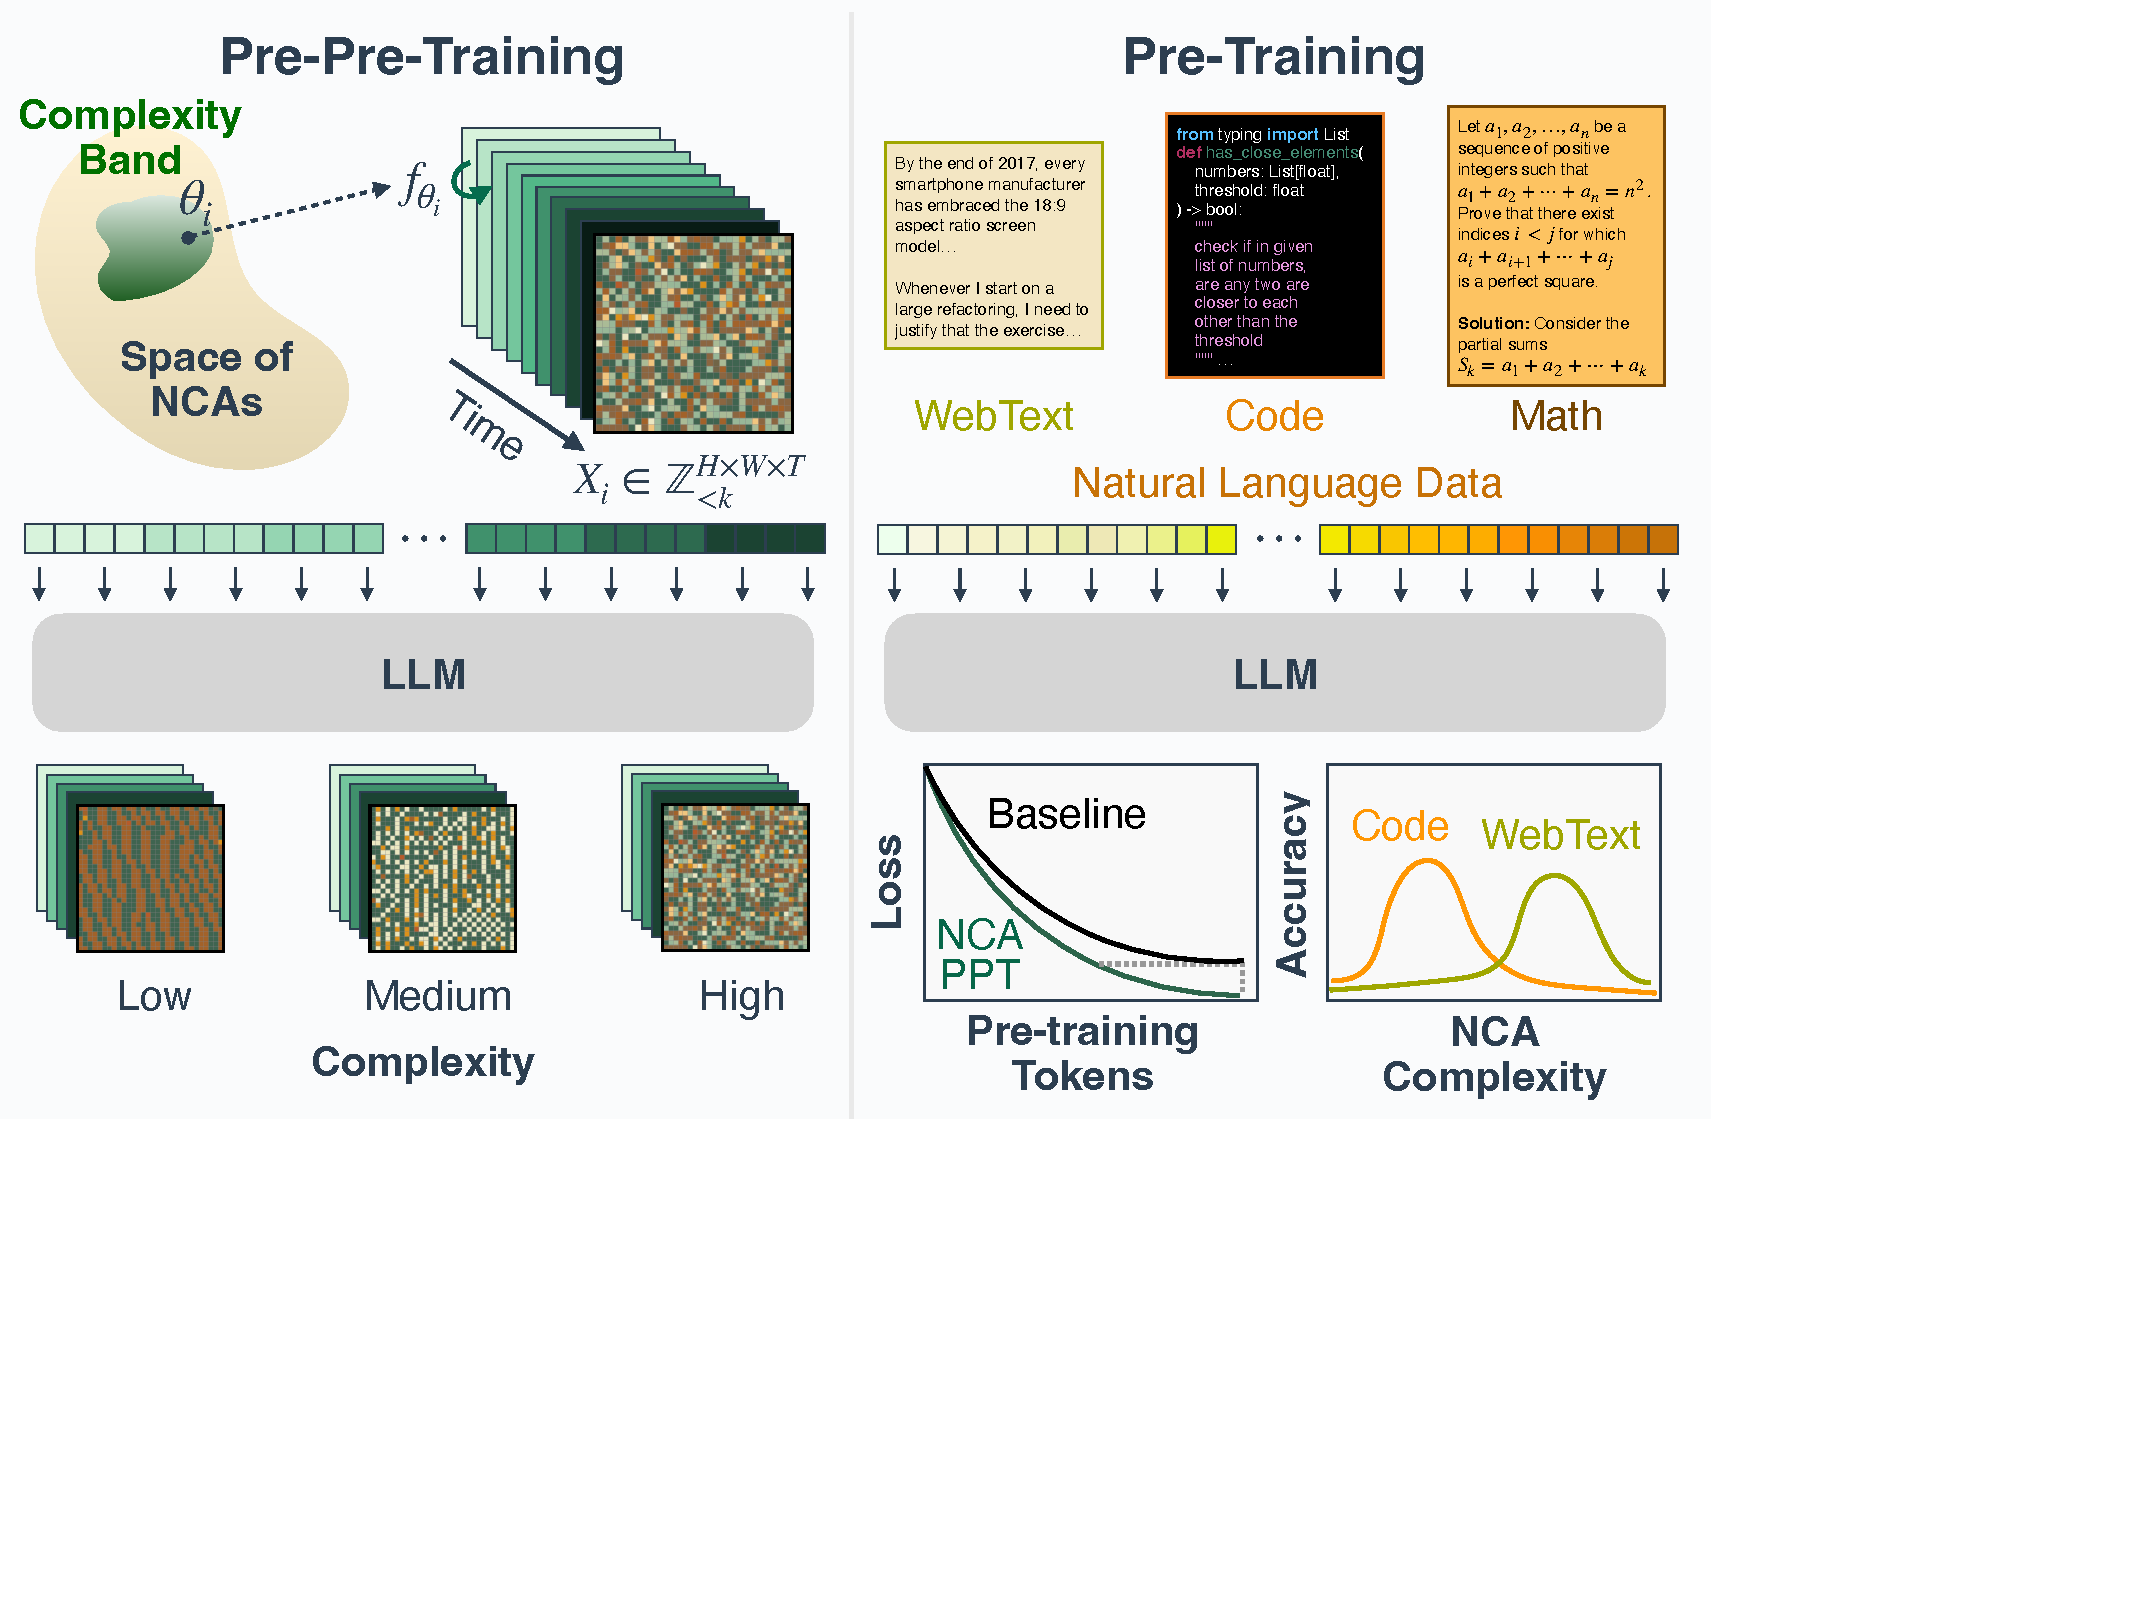
\includegraphics[width=\columnwidth]{figures/LARGER_TEASER.pdf}}
\caption{\textbf{Overview of NCA Pre-pre-training to Language Pre-training.}
We pre-pre-train a transformer with next-token prediction on the dynamics of neural cellular automata (NCA) sampled from selected complexity regions. We then conduct standard pre-training on natural language corpora. NCA pre-pre-training improves both validation perplexity and convergence speed on language pre-training. Interestingly, the optimal NCA distribution varies by downstream domain.}
\label{fig:teaser}
\end{figure}

Scale has transformed neural networks, enabling emergent abilities like reasoning~\citep{jaech2024openai,jiang2023latent, austin2021program} and in-context learning~\citep{brown2020language, wei2022emergentabilitieslargelanguage, zhao2024distributional} in large language models (LLMs). However, neural scaling laws predict that continued improvements require exponentially more data~\citep{kaplan2020scalinglawsneurallanguage}, which is nearing exhaustion by 2028 \citep{villalobos2022will}. Furthermore, natural language inherits many undesirable human biases and needs tedious data curation and cleaning before it is used for training foundation models~\citep{han2025generalintelligencerequiresrewardbased, an2024measuringgenderracialbiases}. This raises a fundamental question: \textbf{Is natural language the only path to learning useful representations?} In this paper, we explore an alternative path to using synthetic data from cellular automata.

Our core hypothesis is that the emergence of reasoning and other abilities in LLMs relies on the underlying structure of natural language, rather than its semantics. Text is a lossy record of human cognition and the world it describes, containing diverse kinds of structure, from reasoning traces to procedural instructions \citep{fractal-language, ruis2024procedural, cheng2025can, delétang2024languagemodelingcompression}. Next-token prediction on such data pressures models to internalize the latent computational processes that support coherent continuations, fostering key capabilities of intelligence \citep{deletang2023language, jiang2023latent}.

If the key ingredient is exposure to various structures rather than language semantics, then richly structured non-linguistic data could also be effective for teaching models to reason. To investigate this hypothesis, we employ algorithmically generated synthetic data from neural cellular automata (NCA) \citep{mordvintsev2020growing} as a synthetic training substrate. NCA generalize systems like Conway's Game of Life \citep{gardner1970mathematical} by replacing fixed dynamics rules with neural networks and can be used to generate diverse data distributions with spatially local rules. This produces long-range spatio-temporal patterns (see Figure \ref{fig:teaser}) of arbitrary sizes that exhibit heavy-tailed, Zipfian token distributions (see Figure~\ref{fig:token-distributions} in Appendix \ref{app:data_distribution_analysis}) reminiscent of natural data.
%--without the semantics. 
Crucially, we propose a method to explicitly control the complexity of NCA, enabling systematic tuning of the synthetic data distribution for optimal transfer to downstream domains. 

Prior work on synthetic pre-training has explored approaches like generating random strings with a recurrent network \citep{bloem2025universalpretrainingiteratedrandom} and simple algorithmic tasks \citep{wu2022insightspretrainingsimplersynthetic, shinnick2025transformers}, but they have yet to match or outperform language training under matched token budgets. We hypothesize this is because such synthetic distributions are narrow and homogeneous, lacking certain key properties that characterize natural language. NCAs address this gap. The parametric structure of NCA yields diverse dynamics and allows systematic control over complexity. This enables us to ask not only whether synthetic data can transfer, but what structural properties make it effective.

We adopt a pre-pre-training framework: an initial phase of training on NCA dynamics that precedes standard pre-training on natural language \citep{hu2025circuitschomskyprepretrainingformal}.
Our ultimate vision is to pre-train entirely on clean synthetic data, followed by fine-tuning on a limited and curated corpora of natural language to acquire semantics \citep{han2025generalintelligencerequiresrewardbased}. The pre-pre-training framework serves as an early prototype of this paradigm, allowing us to measure how computational primitives learned from synthetic NCA transfer to language tasks. Our contributions are as follows: 
% To investigate which structural properties drive transfer, we measure NCA complexity using gzip, which uses the Lempel-Ziv \citep{lempelziv} algorithm and computes an upper bound on Kolmogorov complexity \citep{LiVitanyi2019KC4}. By sampling NCA of different complexity regimes, we study how complexity influences downstream transfer. 


% \dl{Thought: Any way to connect this last sentences in this paragraph as a continuation of the prior, seems like we mention this complexity idea -> motivate pre-pretraining and then come back to this + we mention this in the last sentence of all three of the last 3 paragraphs}

% \dl{My rewrite based on PA comment}
% This motivates our investigation of richly structured non-linguistic sources of data as a training prior. Central to this investigation is the question of what \textit{structural properties} synthetic data should possess to induce transferable representations. Existing work on synthetic data often considers ``synthetic data`` to mean LLM-generated or language-augmented text \citep{qin2025scalinglawssyntheticdata, k2team2025k2v2360openreasoningenhancedllm, Nad__2025, kimiteam2025kimik2openagentic}, which remains tethered to natural language and thus inherits its constraints. We pursue a different, purist approach \citep{shinnick2025transformers, hu2025circuitschomskyprepretrainingformal, bloem2025universalpretrainingiteratedrandom}: synthetic data that is non-linguistic and generated algorithmically.

%Existing work on synthetic data does not answer this question: it considers ``synthetic data'' to mean LLM-generated or language-augmented text \citep{qin2025scalinglawssyntheticdata, k2team2025k2v2360openreasoningenhancedllm, Nad__2025, kimiteam2025kimik2openagentic}, which remains tethered to natural language and thus inherits its constraints. We pursue a different purist approach \citep{shinnick2025transformers, hu2025circuitschomskyprepretrainingformal, bloem2025universalpretrainingiteratedrandom}: synthetic data that is entirely decoupled from natural language and purely generated algorithmically. This allows us to ask not only whether such data can work, but what structural properties make it effective.

% We propose using \textbf{neural cellular automata (NCA)} as a synthetic training substrate. NCAs generalize systems like Conway's Game of Life by replacing fixed rules with neural networks. This parameterization yields a broad diversity of dynamics: NCAs evolve multi-color grids via spatially-local rules, producing \emph{multi-scale}, \emph{long-range} spatiotemporal structure that is easily scalable and well-suited for transfer to language. We adopt a \textbf{pre-pre-training} framework: an initial phase of training that precedes standard pre-training on natural language, with the goal of instilling transferable computational priors before exposure to any linguistic data. In contrast to prior work where synthetic pre-training underperformed natural language, we demonstrate that NCA pre-pre-training yields positive transfer across different language domains and identify the structural properties that make this possible. Our contributions are as follows:

\begin{enumerate}
    \item \textbf{A synthetic pre-pre-training substrate that transfers to language and reasoning.}
    We propose neural cellular automata (NCA) as a fully algorithmic, non-linguistic data source for pre-pre-training. NCA pre-pre-training improves downstream language modeling by up to 6\% and converges up to 1.6$\times$ faster across web text, math, and code. These perplexity gains transfer to reasoning across benchmarks including GSM8K, HumanEval, and BigBench-Lite. Surprisingly, it outperforms pre-pre-training on natural language (C4), even with more data and compute.
    \item{\textbf{Synthetic pre-training enables domain-targeted data design.}}
We find that the optimal NCA complexity regime varies by downstream task: code benefits from lower-complexity rules while math and web text benefit from higher-complexity ones. NCAs' parametric structure offers a new lever for efficient training: tuning the complexity of training distributions to match the computational character of target domains.
    \item \textbf{Attention captures the  most transferable priors.}
 The attention layers capture the most useful computational primitives, accounting for the majority of the transfer gains. Attention appears to be a universal carrier of transferable capabilities such as long-range dependency tracking and in-context learning, whereas MLPs encode more domain-specific knowledge--making MLP transfer conditional on alignment between the synthetic and target domains. 
 
 % These findings align with recent work showing that scaling MLP capacity primarily enhances memorization rather than reasoning \citep{jelassi2025mixtureparrotsexpertsimprove}.


\end{enumerate}


\section{Related Works}

Synthetic data is a broad umbrella term encompassing a wide spectrum of artificially generated data, ranging from using LLMs \citep{Nad__2025,wang2023selfinstructaligninglanguagemodels, xu2025wizardlmempoweringlargepretrained, mukherjee2023orcaprogressivelearningcomplex, li2023textbooksneediiphi15, lu2024mathgeniegeneratingsyntheticdata, wei2019edaeasydataaugmentation} to simple algorithms to generate data.
% In this work, we pursue the latter purist approach to synthetic data that is non-linguistic and generated algorithmically.
In this work, we pursue the latter, a non-linguistic approach.

% \paragraph{LLM-Based Synthetic Data}
% One prominent approach to synthetic data uses existing generative models to produce new data points, such as generating new instructions for training~\citep{wang2023selfinstructaligninglanguagemodels, xu2025wizardlmempoweringlargepretrained}, creating step-by-step reasoning chains~\citep{mukherjee2023orcaprogressivelearningcomplex, li2023textbooksneediiphi15, lu2024mathgeniegeneratingsyntheticdata}, or rephrasing and perturbing existing text~\citep{wei2019edaeasydataaugmentation, karimi2021aedaeasierdataaugmentation, sennrich2016improvingneuralmachinetranslation, ganitkevitch-etal-2013-ppdb}. While effective, these methods remain anchored to natural language distributions.

% One of the most prominent approaches to generating synthetic data is to use an existing generative model to produce new data points~\citep{Nad__2025}.
% This formulation provides a way to more densely sample from the original training distribution~\citep{CITE}, potentially improving coverage and diversity~\citep{CITE}.
% In practice, this often involves using LLMs to generate new instructions, augmentations of the existing data (e.g., rephrasing, token-level perturbation, etc.) \citep{wei2019edaeasydataaugmentation, karimi2021aedaeasierdataaugmentation, sennrich2016improvingneuralmachinetranslation,ganitkevitch-etal-2013-ppdb,lu2024mathgeniegeneratingsyntheticdata}, or entirely new reasoning chains~\citep{wang2023selfinstructaligninglanguagemodels, mukherjee2023orcaprogressivelearningcomplex, li2023textbooksneediiphi15, xu2025wizardlmempoweringlargepretrained}.
% The recent trend of scaling RL during the post-training of LLMs can also be viewed from a synthetic data lens, where the model is rewarded on sampling ``good'' data that meet the success criteria~\citep{}.

\paragraph{Algorithm-Based Synthetic Data}
Some works have gone beyond natural data altogether, using simple algorithmic procedures (e.g., OpenGL shader images) to generate synthetic training data~\citep{baradad2022procedural}. Past works have trained vision models on data generated by simple processes like fractals, dead leaves, and wavelet models~\citep{kataoka2020pre,baradad2021learning,baradad2022procedural}.
Despite lacking semantic content, these models learn representations that transfer well to real images.
\citet{baradad2021learning} argue that what matters is not \textit{natural} data per se, but \textit{naturalistic} data, i.e. data that reproduces the statistical structure of the natural world, such as the approximate scale-invariance ~\citep{field1987relations} or the Zipfian distribution~\citep{zipf1949human,chan2022datadistributionalpropertiesdrive}.

In the language domain, using algorithmically generated data is less common, as language is thought to be uniquely complex.
Nevertheless, some works have explored this approach ~\citep{saxton2019analysingmathematicalreasoningabilities,desai2015programsynthesisusingnatural,papadimitriou2023injecting}.
\citet{chiang2020pretraininglanguagemodelhuman, hu2025between} showed that pre-training LLMs on synthetic data generated by context-free grammars can be useful for natural language modeling. \citet{berkovich2025lifegpt} and \citet{berkovich2025automatagpt} trained LLMs on cellular automata, but did not study the usefulness of the learned representations for language.

\paragraph{Shared Underlying Computation}
A growing body of work suggests that neural networks learn general computations that transfer across domains, raising the possibility that synthetic algorithmic data could instill such primitives directly. \citet{lu2022frozen} show that LLMs trained on natural language can transfer to seemingly unrelated domains like vision and protein folding, and \citet{huh2024platonicrepresentationhypothesis} illustrate that foundation models across different modalities are converging in representation, hinting that they are learning a common structure.
Going further, \citet{mirchandani2023large} show that, even without fine-tuning, LLMs already have in-context learning capabilities for symbolic reasoning, numeric pattern continuation, and robotic control. These works cast LLMs as universal computation engines \citep{lu2022frozen}.
Other works have shown transfer from natural language to robotic RL environments~\citep{reid2022can}.
\citet{zhang2024intelligence} showed that training LLMs on elementary cellular automata allows them to better transfer to chess.

\paragraph{Emergent Complexity}
A central puzzle for algorithmic synthetic data is how simple procedures can give rise to data with rich structure, resembling the complexity of the real world. This echoes a deeper observation about nature itself: despite its diversity, the universe appears governed by simple underlying laws \citep{wigner1990unreasonable, tegmark2008mathematical}, and may even be fundamentally computational \citep{wolfram2020class}. Researchers have developed various measures to quantify such complexity \citep{lloyd2001measures, mitchell2009complexity}, including Kolmogorov complexity \citep{kolmogorov1963tables}, sophistication \citep{mota2013sophistication}, and assembly index \citep{sharma2023assembly}. More recently, epiplexity was introduced as a complexity metric for computationally bounded observers \citep{finzi2026entropy}, demonstrating that simple deterministic rules can produce data useful for learning useful representations. These works suggest that NCAs, despite having simple local rules, can generate arbitrarily complex structures when rolled out over long time horizons, making them a promising source of synthetic training data.

% This shifts the question to how complexity might arise from different computations.
% Early work introduced the concept of edge of chaos~\citep{packard1988adaptation,langton1990computation}, arguing that the most interesting natural and artificial systems lie between predictability and randomness.
% Self-organized criticality~\citep{bak1987self} was one proposed mechanism by which such complexity can emerge~\citep{bak1995complexity}.
% Since then, many researchers have attempted to quantify complexity~\citep{lloyd2001measures,mitchell2009complexity}, including through measures such as Kolmogorov complexity~\citep{kolmogorov1963tables}, sophistication~\citep{mota2013sophistication}, and assembly index~\citep{sharma2023assembly}.
% More recently, epiplexity was introduced as a complexity metric for computationally bounded observers~\citep{finzi2026entropy}, showing how even simple deterministic rules can produce data that is useful for learning properties beyond the rule itself.
% These works suggest that although NCA data has simple rules, when rolled out over long time horizons, it can generate arbitrarily complex structures which are useful to train on~\citep{zhang2024intelligence}.
% Training LLMs requires not only a large amount of data, but the right type of data: it must capture the diversity, complexity, and structural richness of the real world.
% For algorithmic approaches to synthetic data, how could a simple algorithm produce data with this level of complexity?

% Behind its apparent complexity, it is thought that the universe is governed by simple laws~\citep{wigner1990unreasonable,tegmark2008mathematical}, and may even be computational~\citep{wolfram2020class}.
% This shifts the question to how complexity might arise from different computations.
% Early work introduced the concept of edge of chaos~\citep{packard1988adaptation,langton1990computation}, arguing that the most interesting natural and artificial systems lie between predictability and randomness.
% Self-organized criticality~\citep{bak1987self} was one proposed mechanism by which such complexity can emerge~\citep{bak1995complexity}.
% Since then, many researchers have attempted to quantify complexity~\citep{lloyd2001measures,mitchell2009complexity}, including through measures such as Kolmogorov complexity~\citep{kolmogorov1963tables}, sophistication~\citep{mota2013sophistication}, and assembly index~\citep{sharma2023assembly}.
% More recently, epiplexity was introduced as a complexity metric for computationally bounded observers~\citep{finzi2026entropy}, showing how even simple deterministic rules can produce data that is useful for learning properties beyond the rule itself.
% These works suggest that although NCA data has simple rules, when rolled out over long time horizons, it can generate arbitrarily complex structures which are useful to train on~\citep{zhang2024intelligence}.
% In artificial life~\citep{langton1992artificial}, open-endedness has been identified as a property of complexifying systems~\citep{bedau2000open,stanley2015greatness,stanley2017open}.

\section{Method}
\label{sec:method}
We study whether neural cellular automata (NCA) can create training data that teaches transferable computational priors useful for language modeling.

\subsection{Neural Cellular Automata (NCA)}
\label{subsec:nca}

NCA is a generalization of classical cellular automata \citep{WOLFRAM19841}, where the update rule is parametrized as a neural network, allowing the dynamics to be diversely sampled rather than hand-designed.

\paragraph{Random Discrete NCA.}
We use 2D discrete neural cellular automata on a $12{\times}12$ grid with periodic boundaries and a $n=10$ state alphabet, where each cell is represented as a 10-dimensional one-hot vector. The transition dynamics are governed by a neural network $f_\theta$ that maps each cell's $3{\times}3$ neighborhood to logits over next-cell states:
\begin{equation}
c^{(t+1)}_{i} \sim \mathrm{softmax}\!\left(f_\theta\!\left(c^{(t)}_{N(i)}\right) / \tau\right),
\end{equation}
where $c_i^{(t)}$ is the state of cell $i$ at time $t$, $N(i)$ denotes its neighborhood, and $\tau=10^{-3}$ introduces mild stochasticity. We parameterize $f_\theta$ as a $3{\times}3$ convolution (4 channels) followed by a cell-wise MLP with hidden size 16 and ReLU activation, producing 10 logits per cell.

\paragraph{Complexity-based sampling.}
To generate diverse training data, we sample both the transition rules and initial conditions. For each sequence, we randomly initialize the parameters $\theta$ of the transition network and sample the initial grid $c^{(0)}$ i.i.d.\ uniform over $\{0,\dots,9\}$. This procedure yields a distribution over NCA dynamics ranging from trivially predictable (fixed points or short cylce) to highly chaotic and unpredictable.

To sample NCA dynamics with controlled structural complexity, we sample rules based on the gzip compression ratios of generated sequences. For rollouts, we serialize all timesteps into a byte stream and compute $r = \texttt{compressed bytes} / \texttt{raw bytes} * 100$. We retain NCAs with trajectories of $r > 50\%$.

gzip under the hood combines Lempel-Ziv compression ~\citep{lempelziv} with Huffman coding. Since Lempel-Ziv compression provides a computable upper bound on Kolmogorov complexity~\citep{LiVitanyi2019KC4}, gzip compression ratio serves as a practical measure of intrinsic sequence complexity. Compressible sequences exhibit simpler and more predictable structure, whereas incompressible sequences are more chaotic, as seen in Figure~\ref{fig:teaser}. 

%Not all such trajectories provide equally useful learning signal. Ideally, we seek NCA dynamics that exhibit structured complexity akin to natural language--neither trivially regular nor maximally chaotic. Overly simple dynamics (e.g., fixed points or short cycles) are trivially predictable, while fully chaotic systems are fundamentally unpredictable \citep{WOLFRAM19841}. Prior work suggests that the most interesting computations and the richest representations emerge at the ``edge of chaos,'' the critical regime between order and disorder~\citep{NIPS2004_f8da71e5,zhang2024intelligence}. \dl{shorten / edit out complexity / edge of chaos} To operationalize this notion, we use gzip compression ratio~\citep{lempelziv} as a proxy for complexity. Compression ratio directly reflects the spectrum from order to chaos: highly compressible sequences exhibit regular, predictable structure, while incompressible sequences are indistinguishable from random noise. Sequences with intermediate compression ratios occupy the critical regime—structured enough to be learnable, yet complex enough to require non-trivial computational rules to predict. For each rollout, we serialize all timesteps into a byte stream and compute $r = \texttt{compressed\_bytes} / \texttt{raw\_bytes}$, retaining only trajectories with $r > 0.5$.


\subsection{Tokenization}

\paragraph{Patch vocabulary.}
We tokenize each grid using non-overlapping $2{\times}2$ patches, following the patch-based tokenization for vision transformers~\citep{dosovitskiy2021imageworth16x16words}. Each patch contains four cells in $\{0,\dots,9\}$ and is mapped bijectively to an integer token, yielding a fixed vocabulary of $10^4$ patch tokens. We serialize each timestep in row-major order with \texttt{<grid>} and \texttt{</grid>} delimiters, and concatenate timesteps to form sequences of up to 1024 tokens.

\subsection{Training Objective and Interpretation}
We train a transformer autoregressively on the tokenized trajectory $\mathbf{x}=(x_1,\dots,x_N)$ using cross-entropy loss:
\begin{equation}
\mathcal{L} = -\sum_{i=1}^{N} \log p_\phi(x_i \mid x_{<i}).
\end{equation}
Since each sampled $\theta$ defines a distinct dynamics rule, next-token prediction requires inferring the latent rule in context and applying it within the same sequence. This aligns NCA training with the Bayesian view of in-context learning \citep{han2025emergenceeffectivenesstaskvectors, xie2022explanationincontextlearningimplicit}:
% \begin{equation}
% p(x_{t+1}\mid x_{:t}) \approx \int p(x_{t+1}\mid x_t,\theta)\, p(\theta\mid x_{:t})\, d\theta.
% \end{equation}
% \akarsh{not sure you need this last sentence or equation} \ryan{I agree, eq is kinda thrown here with no explanation or variable definitions so it doesn't add anything IMO}

\section{Experimental Setup}
\label{sec:exp_setup}


\subsection{Training Paradigm}
We adopt a three-stage training paradigm \citep{shinnick2025transformers, hu2025circuitschomskyprepretrainingformal, bloem2025universalpretrainingiteratedrandom}:
\begin{enumerate}
    \item \textbf{Pre-pre-training:} An initial training phase designed to instill transferable computational priors before the main pre-training stage. In this work, we propose using synthetic, non-linguistic data (NCA trajectories) for pre-pre-training.
    \item \textbf{Pre-training:} Standard large-scale training on  natural language corpora (web text, code, or math) to acquire linguistic knowledge.
    \item \textbf{Fine-tuning:} Task-specific adaptation (e.g., instruction tuning).
\end{enumerate}
This work studies the transfer from stage 1 to stage 2 and 3: whether computational structure learned from synthetic data can accelerate and improve language model pre-training, and how it manifests in downstream reasoning benchmarks.

\subsection{Setup}
We generate NCA data by randomly sampling neural network weights that define the transition rule. Each trajectory is thus produced by a unique rule, ensuring diversity across the training distribution. We pre-pre-train a Llama-based transformer~\citep{touvron2023llamaopenefficientfoundation} (1.6B parameters, 24 layers, 32 heads, 2048 hidden dimension, weight-tying) on 164M NCA tokens sampled at the $50\%+$ gzip compressibility band, unless otherwise noted. We measure transfer by conducting pre-training on three downstream corpora: OpenWebText~\citep{Gokaslan2019OpenWeb}, OpenWebMath~\citep{paster2023openwebmath}, and CodeParrot~\citep{tunstall2022natural}. We transfer all model weights except the embedding layers, which are re-initialized for the natural language vocabulary. All parameters are updated during pre-training.

For downstream reasoning benchmarks, we evaluate on GSM8K \citep{cobbe2021training}, HumanEval \citep{chen2021evaluating}, and BigBench-Lite \citep{srivastava2023beyond}. We fine-tune the models on the train set for instruction following for GSM8K and BigBench-Lite. We provide the details on our stage 3 pipeline in Appendix~\ref{app:instruction-ft-setup}.

\subsection{Baselines}
We compare against two baselines: (i) \textbf{No pre-pre-training (scratch)}: the model is randomly initialized and trained directly on the pre-training corpora, establishing whether pre-pre-training provides any benefit; (ii) \textbf{Dyck pre-pre-training}: pre-pre-training on K-Dyck, a synthetic formal language studied in \citet{hu2025circuitschomskyprepretrainingformal}, testing how NCA pre-pre-training compares against an alternative synthetic data approach. We generate our pre-pre-training data using $k=128$ and infinite potential depth; (iii) \textbf{C4 pre-pre-training}: pre-pre-training on natural language data (C4; \citet{c4}) with matched token budgets, testing how NCA pre-pre-training compares against natural language pre-pre-training.

\subsection{Hyperparameters}
For both our pre-pre-training and baseline runs, we perform a grid search over learning rate and weight decay and use the best hyperparameters for each method. For pre-training, we train three separate models for a single epoch on each dataset: OpenWebText (9B tokens), OpenWebMath (4B tokens), and CodeParrot (13B tokens). We report the detailed hyperparameters in Table~\ref{tab:hyperparams} in Appendix~\ref{app:experimental-setup}.

For downstream reasoning benchmarks, we use models pre-trained on OpenWebText, OpenWebMath, and CodeParrot for Big-Bench-Lite, GSM8K, and HumanEval, respectively: matching the benchmark domain approximately to the pre-training domain. We report details on fine-tuning in Appendix~\ref{app:instruction-ft-setup}.

\subsection{Evaluation Metrics for Transfer}
We measure the transfer between our pre-pre-training and pre-training by mainly studying validation perplexity on a held-out set and convergence speed \citep{bloem2025universalpretrainingiteratedrandom, hu2025circuitschomskyprepretrainingformal, kaplan2020scalinglawsneurallanguage}. We quantify convergence speed by comparing the number of tokens to reach the final perplexity of the scratch model. On downstream reasoning tasks, our primary evaluation metric is pass accuracy with multiple decodings or pass@$k$ \citep{chen2021evaluatinglargelanguagemodels}. For BigBench tasks, we compute accuracy on a normalized basis to adjust for random guessing associated with multiple-choice questions \citep{srivastava2023beyond}.


% We compare convergence speed by computing the token efficiency metric used in  \citet{hu2025circuitschomskyprepretrainingformal}. Token efficiency gain is defined as: $\text{Token Efficiency Gain} = 1 - \frac{T_{\text{PPT}}^{\text{NCA}} + T_{\text{PT}}^{\text{NCA}}}{T_{\text{PPT}}^{\text{base}} + T_{\text{PT}}^{\text{base}}}$. Where $T_{\text{PPT}}$ represents the number of pre-pre-training tokens and $T_{\text{PT}}$ represents the number of pre-training tokens to achieve the scratch model's final loss. Note that $T_{\text{PPT}}^{\text{base}} = 0$ for the no pre-pre-training baseline.


\section{Results}

We present results on the impact of NCA pre-pre-training on downstream language modeling, and analyze how transfer varies across scale and data complexity.

\begin{figure*}[t]
\centering
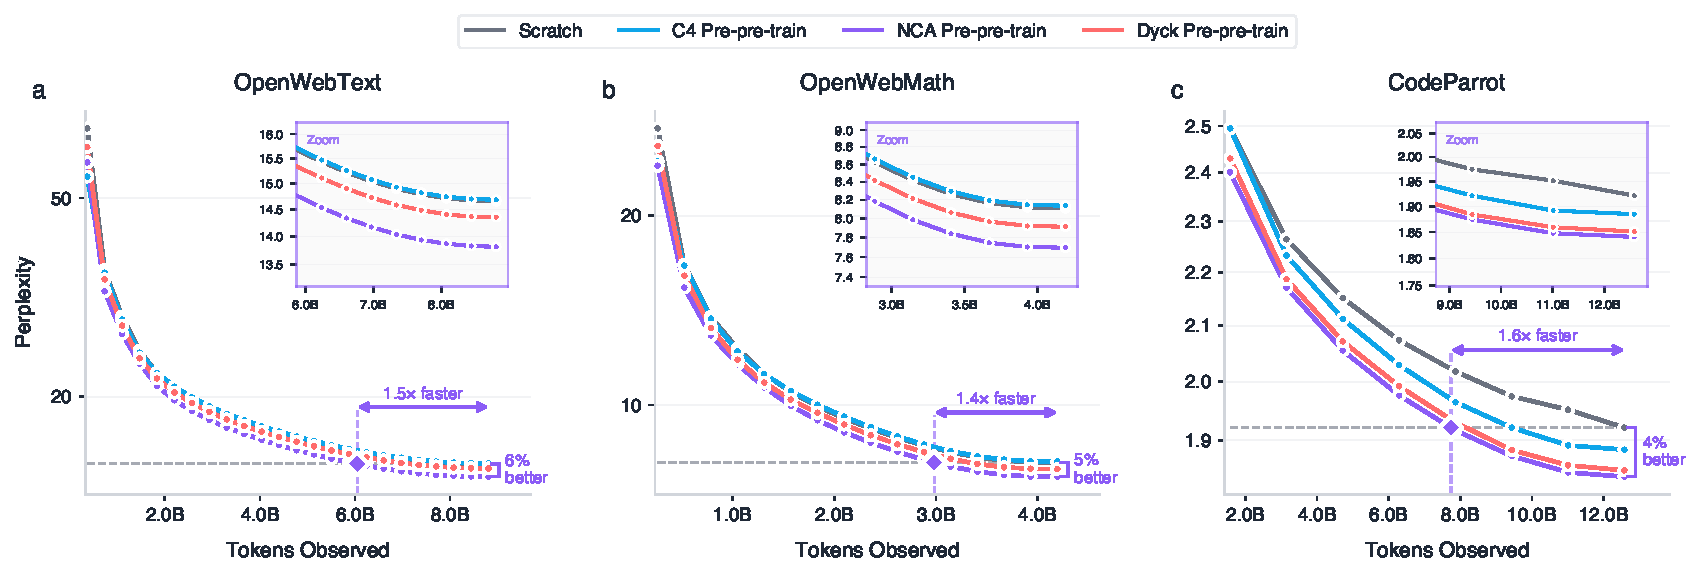
\includegraphics[width=\textwidth]{figures/combined_perplexity_main_dyck.pdf}
\caption{\textbf{NCA pre-pre-training improves and accelerates language model pre-training across diverse domains.} We show the validation perplexity during pre-training on (\textbf{a}) OpenWebText, (\textbf{b}) OpenWebMath, and (\textbf{c}) CodeParrot for 1.6B parameter models. Models pre-pre-trained on NCA trajectories consistently outperform the scratch, Dyck pre-pre-training, and surprisingly even C4 pre-pre-training baselines. NCA pre-pre-training achieves 1.4--1.6$\times$ faster convergence to the scratch baseline's final perplexity while also reaching up to 6\% lower final perplexity. We provide a zoomed-in training curve of the last third of training for clarity.}
\label{fig:combined_perplexity}
\end{figure*}

\subsection{NCA Pre-Pre-Training Improves Language Modeling}
\label{subsec:nca_transfer}

We compare the language modeling performance against three baselines: (i) no pre-pre-training (``scratch''), (ii) pre-pre-training on another natural language dataset C4, and (iii) pre-pre-training on another synthetic language Dyck. 

As seen in Figure~\ref{fig:scaling}, across model scales (400M, 600M, 1.6B) and multiple random seeds, NCA pre-pre-trained models consistently outperform all three baselines (scratch, Dyck, and natural language). On OpenWebText, the best-performing NCA pre-pre-trained 400M model improves downstream perplexity upon the scratch baseline by \textbf{8.6\%}, and the 1.6B model improves by  \textbf{5.7\%}. The relative gain decreases with scale, which is expected as larger models provide a stronger baseline and incremental perplexity improvements become progressively harder to obtain. The improvements nonetheless remain consistent across seeds, indicating that the effect is robust rather than a fragile artifact of initialization.

The most surprising observation is that \textbf{\textit{pre-pre-training on NCA outperforms pre-pre-training on natural language (C4) under matched token and compute budgets}}. To further study this, we compared NCA pre-pre-training (160M tokens) against C4 with significantly more data (1.6B tokens), with and without transferring the pre-trained embedding layers in Figure~\ref{fig:c4-1.6B}. NCA pre-pre-training improves upon this baseline by 5\% on perplexity and converges 1.4$\times$ faster. We hypothesize this reflects what each data source teaches at each scale: C4 may emphasize shallow syntactic patterns, while NCA directly trains long-range dependency tracking and latent rule inference. We return to this discussion in Section \ref{sec:discussion}.

This transfer to natural language holds across the training and generalizes across different domains of math and code, as shown in \cref{fig:combined_perplexity}. These training curves show that NCA pre-pre-training lowers validation perplexity on OpenWebMath and CodeParrot by $4-5\%$ by the end of convergence and with the NCA pre-pre-training we can achieve up to 1.6$\times$ faster convergence. These results demonstrate that the transfer is not specific to a single downstream domain but generalizes across different natural language distributions. This is also not a short-lived initialization effect. The perplexity advantage persists and often grows throughout training, indicating that NCA pre-pre-training genuinely increases token efficiency.
% On average, NCA pre-pre-trained models exhibit token efficiency gains of 31\% on OpenWebText, 27\% on OpenWebMath, and 49\% on CodeParrot to reach equivalent performance.

\subsection{Language Modeling Gains Translate to Downstream Reasoning}
\label{subsec:downstream_tasks}
Perplexity measures language modeling quality, but it is a proxy for the capabilities we ultimately care about. To assess whether these gains translate into task-level improvements, we evaluate on downstream reasoning benchmarks in Table~\ref{table:passk-all}. On GSM8K, NCA pre-pre-training improves accuracy from 3.8\% to 4.4\% at pass@1 and from 36.6\% to 37.9\% at pass@32, with gains growing slightly at higher pass@$k$. On HumanEval, NCA pre-pre-training improves pass@1 but the advantage diminishes at higher k. Interestingly, Dyck pre-pre-training is competitive with NCA on 
HumanEval at higher pass@$k$, and slightly outperforms it at pass@16 
and pass@32. This likely reflects the structural overlap between Dyck languages 
and code, both of which require tracking nesting logic and delimiter patterns. On BigBench-Lite, pass@1 is comparable across all methods, but NCA pre-pre-training outperforms markedly at higher $k$, reaching 36.5\% at pass@4 compared to 29.7\% for C4 and 25.9\% for the scratch baseline. Overall, these results demonstrate that NCA pre-pre-training transfers to downstream reasoning across math, logic, and code.

\begin{figure}[h]
\vskip 0.2in
\centerline{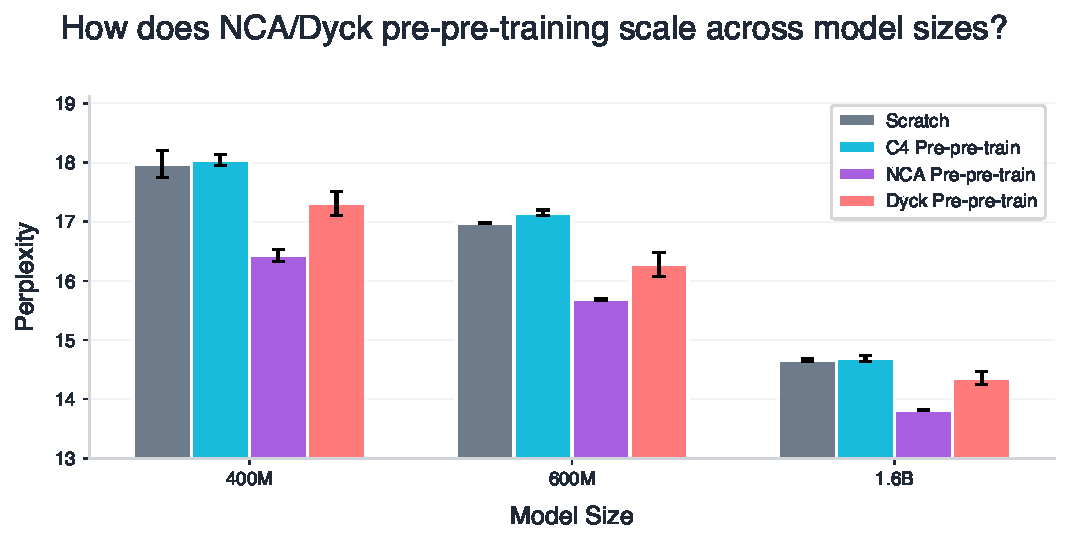
\includegraphics[width=\columnwidth]{figures/4_1_2_dyck.pdf}}
\caption{\textbf{NCA pre-pre-training improves language model training performance across model sizes} (Section \ref{subsec:nca_transfer}). We report the final validation perplexity after pre-training on OpenWebText across (400M, 600M, and 1.6B parameter models). At 164M tokens, C4 pre-pre-training likely acquires shallow syntactic patterns that interfere with downstream learning rather than transferable structure. We investigate this further in Figure \ref{fig:c4-1.6B}.}
\label{fig:scaling}

\end{figure}
\begin{figure}[h]
\vskip 0.2in
\centerline{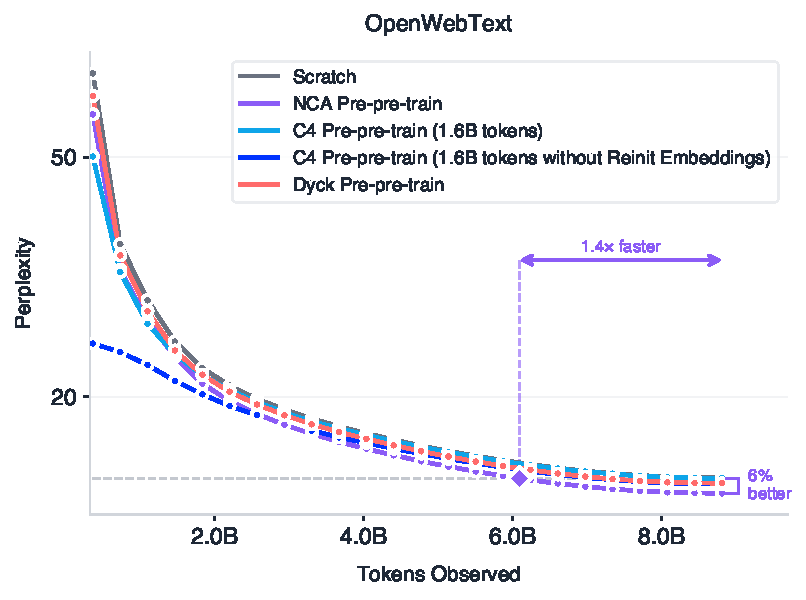
\includegraphics[width=\columnwidth]{figures/owt-c4-50k-large.pdf}}
\caption{\textbf{Pre-pre-training on 160M tokens of NCA is better than pre-pre-training on 1.6B tokens of natural language (C4).} We report the validation perplexity during pre-training on OpenWebText. Perplexity improvement is calculated relative to the C4 pre-pre-trained model. We add a version where we also preserve the embedding layers from pre-pre-training to pre-training (1.6B tokens w/o embedding reinit). Surprisingly even with the embedding layers, NCA pre-pre-training is better.}
\label{fig:c4-1.6B}
\end{figure}

% \begin{table}[ht]
% \centering
% \scriptsize % Smaller font size to fit 5 columns
% \setlength{\tabcolsep}{3pt} % Tighten horizontal padding between columns
% \renewcommand{\arraystretch}{1.2}

% % ---------- GSM8K ----------
% \textbf{Math (GSM8K)} \\
% \begin{tabular}{l c c c c}
% \toprule
% \textbf{pass@$k$} & \textbf{Scratch} & \textbf{C4} & \textbf{NCA} & \textbf{Dyck} \\
% \midrule
% 1   & $3.82\%\pm 0.06\%$ & $3.81\% \pm 0.17\%$ & $\mathbf{4.36\% \pm 0.27\%}$ & $4.10\% \pm 0.40\%$ \\
% 8   & $17.94\% \pm 0.31\%$ & $17.81\% \pm 0.48\%$ & $\mathbf{19.15\% \pm 0.33\%}$ & $18.64\% \pm 0.92\%$ \\
% 16  & $26.47\% \pm 0.46\%$ & $26.29\% \pm 0.64\%$ & $\mathbf{27.77\% \pm 0.25\%}$ & $27.25\% \pm 0.91\%$ \\
% 32  & $36.55\% \pm 0.58\%$ & $36.22\% \pm 0.90\%$ & $\mathbf{37.88\% \pm 0.25\%}$ & $37.42\% \pm 0.73\%$ \\
% \bottomrule
% \end{tabular}

% \vspace{6pt}

% % ---------- HumanEval ----------
% \textbf{Coding (HumanEval)} \\
% \begin{tabular}{l c c c c}
% \toprule
% \textbf{pass@$k$} & \textbf{Scratch} & \textbf{C4} & \textbf{NCA} & \textbf{Dyck} \\
% \midrule
% 1   & $6.75\% \pm 0.56\%$ & $6.27\% \pm 0.26\%$ & $\mathbf{7.49\% \pm 0.38\%}$ & $6.92\% \pm 0.09\%$ \\
% 8   & $11.16\% \pm 0.59\%$ & $10.49\% \pm 0.52\%$ & $\mathbf{11.43\% \pm 0.81\%}$ & $11.33\% \pm 0.18\%$ \\
% 16  & ${12.56\% \pm 0.57\%}$ & $11.58\% \pm 0.59\%$ & $12.55\% \pm 0.89\%$ & $\mathbf{12.78\% \pm 0.24\%}$ \\
% 32  & ${13.85\% \pm 0.51\%}$ & $12.56\% \pm 0.69\%$ & $13.78\% \pm 1.04\%$ & $\mathbf{14.29\% \pm 0.41\%}$ \\
% \bottomrule
% \end{tabular}

% \vspace{6pt}

% % ---------- BigBench-Lite ----------
% \textbf{Reasoning (BigBench-Lite)} \\
% \begin{tabular}{l c c c c}
% \toprule
% \textbf{pass@$k$} & \textbf{Scratch} & \textbf{C4} & \textbf{NCA} & \textbf{Dyck} \\
% \midrule
% 1   & $23.25\% \pm 2.46\%$ & $24.46\% \pm 2.68\%$ & $\mathbf{25.95\% \pm 0.45\%}$ & $24.07\% \pm 1.12\%$ \\
% 8   & $46.28\% \pm 1.64\%$ & $47.37\% \pm 1.96\%$ & $\mathbf{48.47\% \pm 0.44\%}$ & $46.21\% \pm 1.24\%$ \\
% 16  & $49.39\% \pm 1.60\%$ & $50.53\% \pm 1.92\%$ & $\mathbf{51.50\% \pm 0.51\%}$ & $49.06\% \pm 1.41\%$ \\
% 32  & $51.74\% \pm 1.65\%$ & $52.76\% \pm 1.82\%$ & $\mathbf{53.65\% \pm 0.53\%}$ & $51.15\% \pm 1.54\%$ \\
% \bottomrule
% \end{tabular}

% \caption{\textbf{NCA pre-pre-training improves performance on downstream reasoning benchmarks.} We report the mean pass@$k$ $\pm$ std over 4 training seeds.}
% \label{table:passk-all}
% \end{table}

\begin{table}[ht]
\centering
\scriptsize % Smaller font size to fit 5 columns
\setlength{\tabcolsep}{3pt} % Tighten horizontal padding between columns
\renewcommand{\arraystretch}{1.2}
% ---------- GSM8K ----------
\textbf{Math (GSM8K)} \\
\begin{tabular}{l c c c c}
\toprule
\textbf{pass@$k$} & \textbf{Scratch} & \textbf{C4} & \textbf{NCA} & \textbf{Dyck} \\
\midrule
1   & $3.8\%\pm 0.1\%$ & $3.8\% \pm 0.2\%$ & $\mathbf{4.4\% \pm 0.3\%}$ & $4.1\% \pm 0.4\%$ \\
8   & $17.9\% \pm 0.3\%$ & $17.8\% \pm 0.5\%$ & $\mathbf{19.2\% \pm 0.3\%}$ & $18.6\% \pm 0.9\%$ \\
16  & $26.5\% \pm 0.5\%$ & $26.3\% \pm 0.6\%$ & $\mathbf{27.8\% \pm 0.3\%}$ & $27.3\% \pm 0.9\%$ \\
32  & $36.6\% \pm 0.6\%$ & $36.2\% \pm 0.9\%$ & $\mathbf{37.9\% \pm 0.3\%}$ & $37.4\% \pm 0.7\%$ \\
\bottomrule
\end{tabular}
% \vspace{6pt}
% ---------- HumanEval ----------
\textbf{Coding (HumanEval)} \\
\begin{tabular}{l c c c c}
\toprule
\textbf{pass@$k$} & \textbf{Scratch} & \textbf{C4} & \textbf{NCA} & \textbf{Dyck} \\
\midrule
1   & $6.8\% \pm 0.6\%$ & $6.3\% \pm 0.3\%$ & $\mathbf{7.5\% \pm 0.4\%}$ & $6.9\% \pm 0.1\%$ \\
8   & $11.2\% \pm 0.6\%$ & $10.5\% \pm 0.5\%$ & $\mathbf{11.4\% \pm 0.8\%}$ & $11.3\% \pm 0.2\%$ \\
16  & ${12.6\% \pm 0.6\%}$ & $11.6\% \pm 0.6\%$ & $12.6\% \pm 0.9\%$ & $\mathbf{12.8\% \pm 0.2\%}$ \\
32  & ${13.9\% \pm 0.5\%}$ & $12.6\% \pm 0.7\%$ & $13.8\% \pm 1.0\%$ & $\mathbf{14.3\% \pm 0.4\%}$ \\
\bottomrule
\end{tabular}
% \vspace{6pt}
% ---------- BigBench-Lite ----------
\textbf{Reasoning (BigBench-Lite)} \\
\begin{tabular}{l c c c c}
\toprule
\textbf{pass@$k$} & \textbf{Scratch} & \textbf{C4} & \textbf{NCA} & \textbf{Dyck} \\
\midrule
1 & $15.4\% \pm 1.1\%$ & $\mathbf{15.9\% \pm 0.9\%}$ & $15.0\% \pm 1.2\%$ & $13.4\% \pm 2.8\%$ \\
2 & $20.9\% \pm 2.5\%$ & $22.8\% \pm 1.2\%$ & $\mathbf{26.5\% \pm 1.0\%}$ & $18.1\% \pm 2.3\%$ \\
4 & $25.9\% \pm 3.9\%$ & $29.7\% \pm 1.3\%$ & $\mathbf{36.5\% \pm 2.1\%}$ & $22.7\% \pm 2.1\%$ \\
\bottomrule
\end{tabular}
\caption{\textbf{NCA pre-pre-training improves performance on downstream reasoning benchmarks.} We report the mean pass@$k$ $\pm$ std over 4 training seeds.}
\label{table:passk-all}
\end{table}

\subsection{What Drives Transfer?}
\label{subsec:what_drives}

The preceding results establish that NCA pre-pre-training improves both language modeling and reasoning. We now investigate the mechanism: which model components capture the transferable structure, and what properties of the synthetic data control transfer effectiveness?

\subsubsection{Attention captures the most transferable primitives.}
\label{subsubsec:attn_transfer}
To isolate which model components carry the transfer signal, we selectively re-initialize subsets of weights after NCA pre-pre-training and measure the impact on language modeling. As shown in Figure~\ref{fig:reinit_layers}, re-initializing attention weights causes the largest degradation in transfer across all configurations, indicating that attention captures the most transferable computational primitives.

The role of other components is more nuanced. On OpenWebText, retaining MLP and LayerNorm weights degrades transfer, suggesting these layers encode NCA-specific statistics that interfere with language learning. On CodeParrot, these components have negligible effect. This asymmetry suggests that attention is more transferable across domains, whereas MLP layers are contingent on whether the domain-specific priors align with the target task.

These findings align with concurrent work identifying attention as the primary locus of transferable structure in synthetic pre-training \citep{shinnick2025transformers, shinnick2025learnimagesproceduralwarmup}. They also resonate with recent analyses of Mixture-of-Expert architectures, which demonstrate that scaling MLP parameters primarily enhance memorization rather than reasoning \citep{jelassi2025mixtureparrotsexpertsimprove}. Together, these results suggest a functional division: attention layers learn general-purpose mechanisms for tracking dependencies and inferring latent rules, while MLP layers specialize in storing domain-specific patterns and statistics. This division may explain why attention transfers universally from NCA to language, whereas MLP weights can introduce interference when the source and target domains differ substantially.

\begin{figure}[ht]
\vskip 0.2in
\centerline{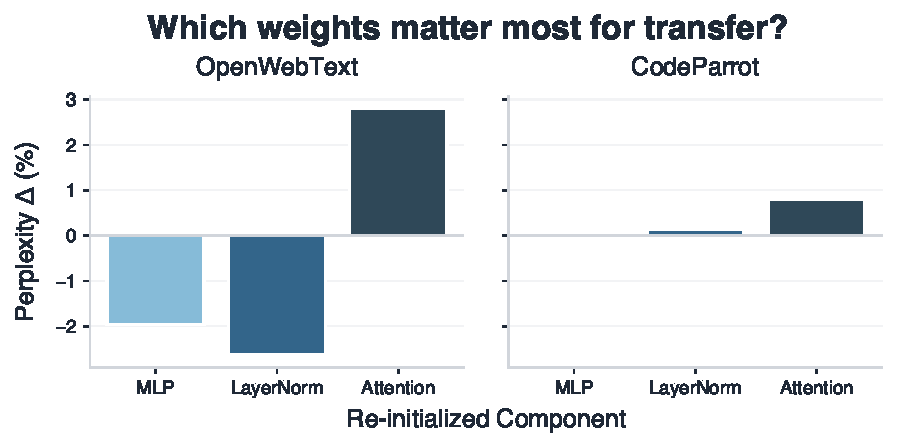
\includegraphics[width=\columnwidth]{figures/combined_reinit_bar.pdf}}
\caption{\textbf{Attention weights are most crucial for positive transfer.} We report the change in validation perplexity when selectively re-initializing model components after NCA pre-pre-training, relative to full transfer. Higher means the component is more important for transfer. Re-initializing attention causes the largest degradation across both OpenWebText and CodeParrot, while MLP and LayerNorm effects are domain-dependent.}
\label{fig:reinit_layers}
\end{figure}

\subsubsection{Data complexity modulates transfer and the optimum is domain-dependent.}

Having established that attention carries the most transferable signal, we next ask: what properties of NCA data affect the transfer? We analyze complexity along two complementary axes: gzip compressibility (as an upper bound to Kolmogorov complexity) and alphabet size $n$ (size of the state space).

\paragraph{Complexity via gzip.} We generate NCA trajectories of varying gzip compressibility bands (20–30\%, 30–40\%, 40–50\%, 50\%+). Smaller compression ratios imply regular, low-entropy dynamics that are more predictable, whereas larger compression ratios generate more diverse and unpredictable trajectories with richer spatiotemporal structure, as illustrated in \cref{fig:teaser}.

As shown in Figure~\ref{fig:gzip_bands}, the optimal complexity band varies by downstream domain. OpenWebText benefits from less compressible (more complex) NCA rules in the 50\%+ band, while CodeParrot shows a sweet spot at intermediate complexity (30–40\% gzip). Strikingly, this aligns with the intrinsic complexity of the target corpora themselves in Figure~\ref{fig:token-distributions} of Appendix~\ref{app:data_distribution_analysis}: OpenWebText and OpenWebMath have gzip ratios of 60–70\%, whereas CodeParrot is substantially more compressible at 32\%. The correlation is somewhat direct. Domains with higher intrinsic complexity benefit from higher-complexity synthetic data, and vice versa. This suggests a plausible and practical principle: \textbf{matching the complexity of synthetic pre-training data to the target domain maximizes transfer}.

\begin{figure}[ht]
\vskip 0.2in
\centerline{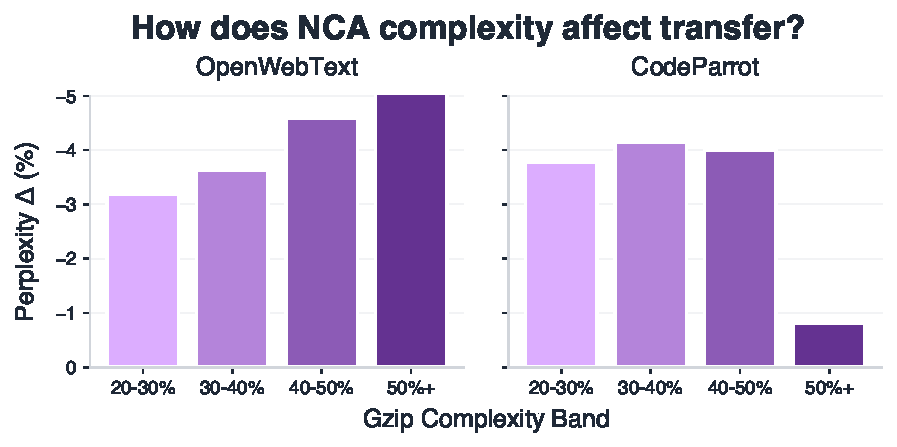
\includegraphics[width=\columnwidth]{figures/combined_complexity_transfer.pdf}}
\caption{\textbf{Optimal NCA complexity is domain-dependent.} We report the validation perplexity change of models trained with different NCA complexities from the scratch model. OpenWebText benefits from higher-complexity data (50\%+), while CodeParrot peaks at intermediate complexity (30–40\%). This suggests that matching synthetic data complexity to the target domain is necessary to maximize transfer.}
\label{fig:gzip_bands}
\end{figure}

\textbf{Rule space expressiveness via alphabet size.} We vary the NCA state alphabet $n \in \{2, 10, 15\}$, which controls the diversity of possible local interactions. As shown in Figure~\ref{fig:nca_u_curve}, larger alphabets ($n=10, 15$) exhibit diminishing returns: performance improves the most at an intermediate NCA token budget, then the improvement gap narrows. Surprisingly, the smallest alphabet ($n=2$) scales most favorably, continuing to improve where larger alphabets plateau. 

As seen in Figure~\ref{fig:nca_gzip} in Appendix~\ref{app:data_distribution_analysis}, when increasing $n$, the resulting NCA data naturally becomes more complex. This result suggests that although larger rule spaces can express more complex dynamics, better guidance is necessary to sample a diverse set of NCAs that optimally transfer to language. Thus, constraining the space to $k{=}2$ may paradoxically help by concentrating samples on dynamics with more consistent, transferable structure.
    
\begin{figure}[h]
\vskip 0.2in
\centerline{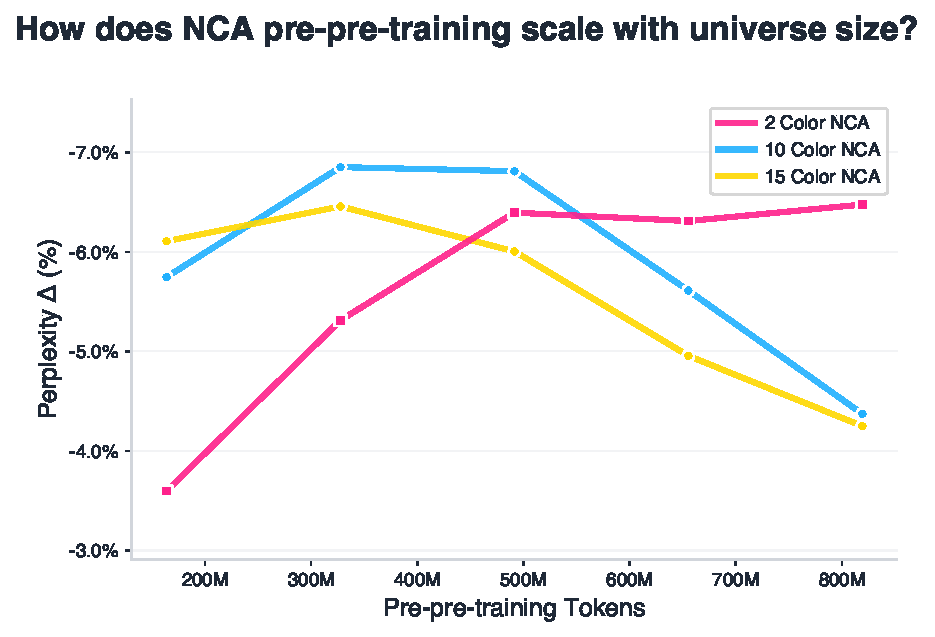
\includegraphics[width=\columnwidth]{figures/stages_of_pt.pdf}}
\caption{\textbf{NCA alphabet size changes scaling behavior.} We report the perplexity change relative to the scratch model (higher is better) on OpenWebText across different alphabet sizes $n$ and NCA pre-pre-training token budgets. NCA improves perplexity at all token budgets. The smaller alphabet scales better, and the improvements degrade with scale for larger alphabets.}
\label{fig:nca_u_curve}
\end{figure}

Together, these results indicate that transfer is not simply ``more NCA data is better.'' The complexity of synthetic data, both gzip and alphabet size, must be calibrated. This offers a lever unavailable in natural language pre-training: the ability to tune the training distribution to match the computational character of target domains.
We further discuss the implications for domain-targeted pre-training in Section~\ref{sec:discussion}.


\section{Discussion}
\label{sec:discussion}

\paragraph{Why should we expect transfer?}
NCA data are substantially different from natural language and generated by deterministic processes, prompting the question of why one should expect transfer at all? We argue that NCAs may provide a purer training signal for in-context rule inference. In natural language, models may rely on semantic ``shortcuts'' or co-occurrence priors \citep{abbas2023semdedupdataefficientlearningwebscale, geirhos2020shortcut}. 
In contrast, every NCA sequence is generated by a hidden transition rule -- parameterized by a random neural network. With no semantic knowledge to fall back on, every NCA token guides the model to in-context rule inference \citep{kirsch2022general}.

This mirrors a core capability required for language modeling~\citep{brown2020language, wei2022emergentabilitieslargelanguage, dong2024survey}. \citet{xie2022explanationincontextlearningimplicit} show that training on natural text teaches models to perform implicit Bayesian inference over latent concepts: each sequence draws from a latent concept, and predicting the next token means conditioning on the inferred concept. The same mechanism appears in math and code as well \citep{garg2023transformerslearnincontextcase, cook2025programming}. Prior work on formal languages and algorithmic tasks such as Dyck and string copying \citep{hu2025circuitschomskyprepretrainingformal, wu2022insightspretrainingsimplersynthetic,shinnick2025learnimagesproceduralwarmup} also train for this kind of in-context inference. Unlike these tasks, NCAs encompass a broad, universal class of computable functions \citep{Copeland2012}, some of which realize Turing-complete systems \citep{Rendell2002, wolfram2003new}.
The breadth and scale of this distribution makes memorization infeasible, forcing models to learn a general mechanism for rule inference \citep{li2024languagemodelslearncontext} that applies across the function class.

This framing is supported by our mechanistic finding from Section~\ref{subsubsec:attn_transfer}: attention layers, not the MLPs or LayerNorms carry the most transferable structure. \citep{olsson2022context} showed that ICL ability emerges with the formation of \textit{induction heads} -- attention circuits that help copy information from previous tokens to future ones. Because NCA pre-pre-training exclusively rewards this behavior, it may induce earlier and more robust formation than language-only pre-training. The transferred attention weights are, in effect, the in-context learning circuits, which are later adapted for downstream tasks and domains.

A secondary motivation for transfer is \textit{epiplexity} \citep{finzi2026entropy}. Classical information theory suggests deterministic transformations cannot increase information content \citep{Polyanskiy_Wu_2025}, thus questioning whether LLMs can learn meaningful structure from NCAs.
However, this view assumes a computationally unbounded observer. For computationally bounded observers, \citet{finzi2026entropy} show that deterministic processes can generate useful structural information--coined epiplexity--that models must internalize to learn useful representations of the data.
Their key insight is that simple local rules, like CA, can produce emergent structures (e.g., gliders, collisions) that a finite-capacity model cannot brute-force simulate. Instead, the model must learn a representation that allows it to predict the simulation at a coarser-grained abstraction. Learning these representations over a diverse and universal class of functions like NCA may help with learning representations of natural language as well.


\paragraph{Why is 160M tokens of automata better than 1.6B tokens of text?}

Surprisingly, with a significantly lower token budget, pre-pre-training on NCA data improves language modeling more than pre-pre-training on natural language (C4), as shown in Figure~\ref{fig:combined_perplexity}.
How can abstract dynamical systems' data transfer better to language than language itself?


Even at 1.6B tokens, natural language pre-pre-training remains in an early training regime. Compute-optimal scaling laws suggest \citep{hoffmann2022trainingcomputeoptimallargelanguage} that a 1.6B parameter model requires roughly 32B tokens.
At this early stage, language models primarily acquire shallow, local patterns and only learn more complex structures later on~\citep{evanson2023language,chen2023sudden}.

With limited tokens, C4 pre-pre-training likely spends most of its capacity on these surface-level regularities rather than the long-range dependencies and in-context learning that transfer broadly.

In contrast, we hypothesize that NCA sequences provide a purer training signal for in-context learning. Each sequence is generated by a single latent rule that the model must infer from context and then apply consistently. Once identified, next-token prediction becomes nearly deterministic. 

Moreover, NCA pre-pre-training introduces a form of diversity orthogonal to what additional language tokens would provide. Despite their scale, many natural language datasets exhibit substantial redundancy \citep{abbas2023semdedupdataefficientlearningwebscale} in linguistic patterns and topic coverage. Since each of our NCA sequences represents a unique function to model, this diversity may be more efficient per token at building general-purpose representations.


\paragraph{Beyond one-size-fits-all pre-training}

Our complexity ablations reveal a nuanced picture that the optimal distribution for training varies by downstream domain. In \cref{fig:gzip_bands}, we observed that code benefits from lower-complexity NCA rules, while web text and math benefit from higher-complexity ones, suggesting these domains encode computations of measurably different character. This opens a new axis of control. Rather than treating training data as fixed, we can tune the structures of synthetic data to match the target domain. Unlike grammar-based synthetic tasks, where each formal grammar defines a task with fixed structural complexity, NCAs provide a continuous and tunable spectrum of complexity within a single generator family. If researchers can craft distributions that embody the primitives a domain requires (e.g., rigid state-tracking for code \citep{li2025codeiocondensingreasoningpatterns}, richer long-range dependencies for genomic sequences \citep{wu2025generatorlongcontextgenerativegenomic}), they can instill these capabilities directly, without scaling to trillions of general-purpose tokens.
The result could aid the development of specialized, small language models \citep{belcak2025smalllanguagemodelsfuture} that are more efficient to train and deploy---trained not on more data, but on better-matched data.
% Our framework positions NCA pre-pre-training as a complement to, not a replacement for, standard language pre-training. Our hypothesis that aligns with that of \citet{finzi2026entropy} is that training on structural information enables computationally bounded observers to extract reusable circuits that transfer across domains. Thus, once strong computational priors are learned from synthetic data like NCA, models can quickly acquire domain-specific semantics from limited clean data. 
\paragraph{Limitations and open problems}
\label{subsec:limits_scaling_nca}

A key question is whether NCA data can serve not only as a pre-pre-training signal, but as a scalable substitute for natural language pre-training. For larger alphabet sizes ($n=10,15$), we observe a reverse U-shaped trend: downstream improvement is optimal up to an intermediate token budget but plateaus beyond it. This behavior nonetheless reinforces our central thesis: effective synthetic pre-training depends critically on structural choices in the data generator, not merely on scale. 

% The fact that increasing synthetic data alone is insufficient suggests that calibrated distributions and complexity regimes matter more than volume, and motivates future work on principled methods for tuning synthetic generators to match target domain structure. We also only study two axes that characterize complexity, but 


This points to a key open problem for future work: developing principled methods to guide synthetic generators to sample structures that match those of target domains. Our complexity results demonstrate that such matching matters, but gzip compressibility and alphabet size are only two lens on complexity. Complexity is multifaceted: a sequence can be compressible yet be rich in long-range dependencies, or vice versa. Characterizing which axes of complexity (e.g., size of NCA network, grid size, or epiplexity) matter for which domains and learning to sample synthetic data accordingly could unlock fully synthetic pre-training at scale.

NCA represents one point in the vast space of possible synthetic data generators. The key insight from our work is not that NCA specifically is optimal, but that structured synthetic data with appropriate complexity characteristics can provide meaningful pre-training signal even without any linguistic content. The question is no longer whether synthetic pre-training can work, but how to design synthetic data distributions that maximize what models learn.

% \dl{Draft of the point from NCA as not the best source point}
% Finally, while NCAs can generate a massive universe of dynamics and structure, they are only one of many possible mechanisms to generate rich structured non-linguistic data. Beyond diversity and scale, NCAs do not provide a fundamentally unique source of structure from alternatives. From a scalability standpoint, mixing and layering various other sources of computational tasks may be a promising direction for amplifying the pre-pretraining signal we observe.

% \section{Conclusion}
% \pulkit{Merge discussion and conclusion into one.}
% Natural language has been the default substrate for training language models, but it is an imperfect one. Internet text entangles knowledge with reasoning, and naturally comes with systemic biases and potentially harmful content. Our results suggest an alternative: if the primitives that matter for language modeling, such as rule inference, state tracking, and long-range dependency modeling, can be acquired from abstract and easily-controllable dynamical systems, we can decouple what models learn from where they learn it. This opens the possibility of foundation models that acquire reasoning without inheriting human biases from inception, trained on data we fully control. The question is no longer whether synthetic pre-training can work, but how far it can go.

% \sw{let's add that NCA is probably not the best synthetic data, but one of them either in limitations or conclusion}

%restatable

% \section*{Accessibility}
% Authors are kindly asked to make their submissions as accessible as possible for everyone including people with disabilities and sensory or neurological differences.
% Tips of how to achieve this and what to pay attention to will be provided on the conference website \url{http://icml.cc/}.

% \section*{Software and Data}

% If a paper is accepted, we strongly encourage the publication of software and data with the
% camera-ready version of the paper whenever appropriate. This can be
% done by including a URL in the camera-ready copy. However, \textbf{do not}
% include URLs that reveal your institution or identity in your
% submission for review. Instead, provide an anonymous URL or upload
% the material as ``Supplementary Material'' into the OpenReview reviewing
% system. Note that reviewers are not required to look at this material
% when writing their review.

% Acknowledgements should only appear in the accepted version.
% \section*{Acknowledgements}

% \section*{Impact Statement}
% This paper presents work whose goal is to advance the field of 
% Machine Learning. There are many potential societal consequences 
% of our work, none which we feel must be specifically highlighted here.

\section*{Author Contributions}
\textbf{Dan Lee} co-lead the project and contributed to all aspects of experiments and writing.

\textbf{Seungwook Han} co-lead the project and contributed to all aspects of experiments and writing.

\textbf{Akarsh Kumar} supported this project, contributed to the design of the experiments and significantly to the writing.

\textbf{Pulkit Agrawal} advised the development of the project idea from inception and contributed significantly to the writing.




\section*{Acknowledgment}
We want to express our gratitude to Zachary Schinnick, Phillip Isola, Yoon Kim, Ryan Bahlous-Boldi, Idan Shenfeld, Nitish Dashora, and members of the Improbable
AI lab for the helpful discussion on the paper. We are grateful to MIT Supercloud and the Lincoln Laboratory Supercomputing Center for providing HPC resources. The
research was supported in part by NSF CSGrad4US Fellowship, Google, and Amazon. Also, the research was sponsored by the Army Research Office and was accomplished under Grant Number W911NF-23-1-0277. The views and conclusions contained
in this document are those of the authors and should not
be interpreted as representing the official policies, either
expressed or implied, of the Army Research Office, Naval
Research Office, Air Force, or the U.S. Government


\bibliography{references}
\bibliographystyle{icml2025}


%%%%%%%%%%%%%%%%%%%%%%%%%%%%%%%%%%%%%%%%%%%%%%%%%%%%%%%%%%%%%%%%%%%%%%%%%%%%%%%
%%%%%%%%%%%%%%%%%%%%%%%%%%%%%%%%%%%%%%%%%%%%%%%%%%%%%%%%%%%%%%%%%%%%%%%%%%%%%%%
% APPENDIX
%%%%%%%%%%%%%%%%%%%%%%%%%%%%%%%%%%%%%%%%%%%%%%%%%%%%%%%%%%%%%%%%%%%%%%%%%%%%%%%
%%%%%%%%%%%%%%%%%%%%%%%%%%%%%%%%%%%%%%%%%%%%%%%%%%%%%%%%%%%%%%%%%%%%%%%%%%%%%%%
\newpage
\appendix
\onecolumn

\section{Analysis on Natural and Synthetic Data Distributions}
\label{app:data_distribution_analysis}

\begin{figure}[h]
    \centering
    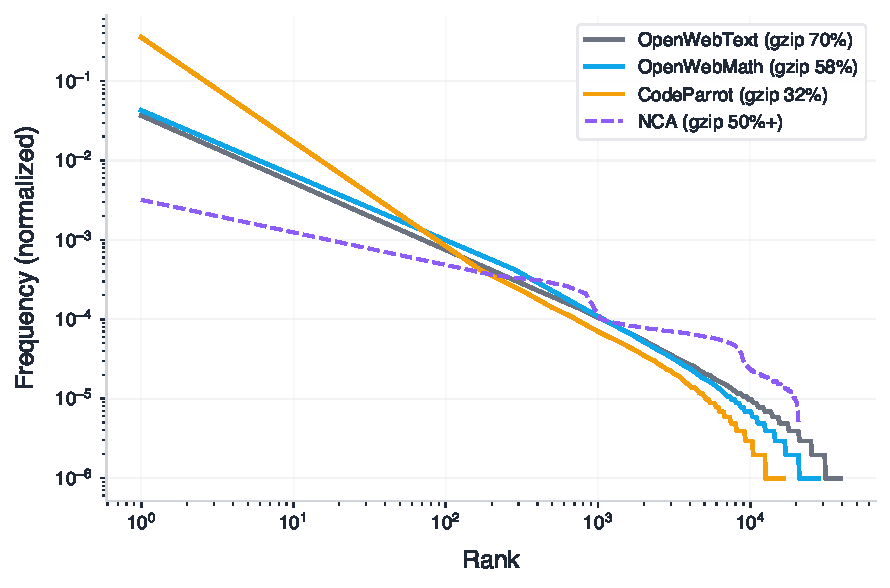
\includegraphics[width=0.5\linewidth]{figures/token_distribution.pdf}
    \caption{\textbf{NCA data exhibits a similar Zipfian or power-law structure to natural language.} We compare the relative token frequency distribution for each of the natural language corpora and NCA data. Natural language from different domains has different average complexity as measured by gzip compressibility (see legend).}
    \label{fig:token-distributions}
\end{figure}

\begin{figure}[t]
    \centering
    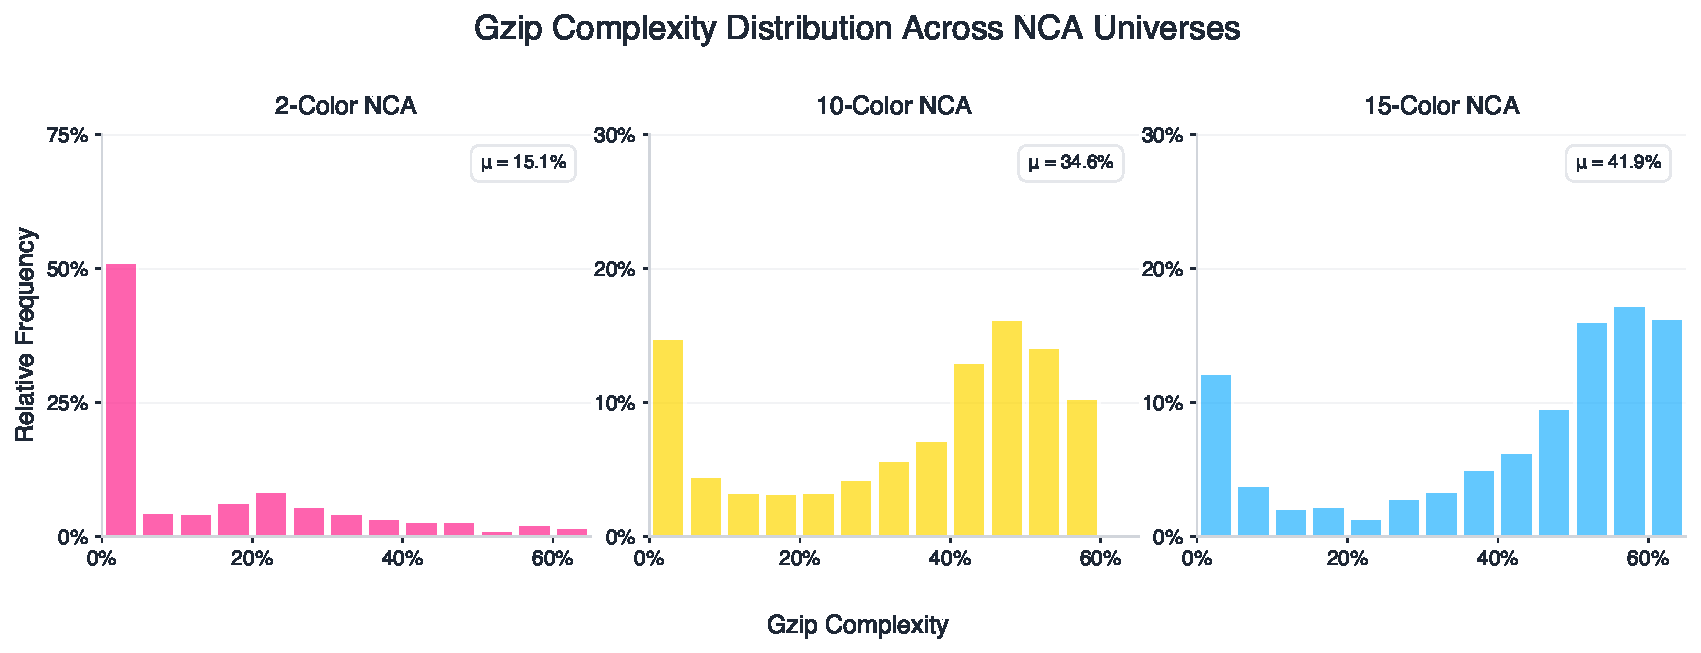
\includegraphics[width=\linewidth]{figures/gzip_complexity_distribution.pdf}
    \caption{Different NCA alphabet sizes, $n=2,10,15$ naturally yield different complexity distributions of the data. Increasing $n$ inherently increases the complexity of the data.}
    \label{fig:nca_gzip}
\end{figure}

In this section, we examine the distributions of natural-language and NCA-generated synthetic data with respect to two primary high-order heuristics: (1) token frequency distribution and (2) gzip compressibility.
\subsection{NCA data exhibits similar token distributions to natural language}
To compare the token frequency across different data distributions, we sample and tokenize random text sequences from the natural language datasets (OpenWebText, OpenWebMath, and CodeParrot) and NCA generated data ($n=15$). Figure~\ref{fig:token-distributions} shows the distribution of relative token frequencies. Data generated from the NCAs follows a heavy-tailed, Zipfian token distribution that is structured similarly to natural language. Another interesting observation is that natural language depending on the domain varies quite drastically from 32\% in code and 60-70\% in math and web text.

\subsection{Increasing the vocabulary size $n$ leads to more complex generated trajectories}
Figure~\ref{fig:nca_gzip} compares the distribution of gzip complexity across trajectories generated by randomly sampled NCAs across different alphabet sizes $n=2,10,15$. As $n$ increases, the distribution skews towards less compressible, more complex data. This implies that with higher $n$, the universe of rules expands and naturally the dynamics become more complex.

% \dl{Thought here: This could imply (1) that GZIP isn't as good of a metric for distinguishability at high $n$ or (2) high $n$ have more complex sequences and rules.}
\section{Detailed Pre-pre-training and Pre-training Setup}
\label{app:experimental-setup}

Table~\ref{tab:hyperparams} summarizes the hyperparameters used for both pre-pre-training on NCA data and subsequent pretraining on natural language datasets. We sweep various batch sizes (32 to 512), learning rates ($1\times10^{-3}$ to $1\times10^{-5}$), and weight decays ($1\times10^{-4}$ to $1\times 10^{-6}$). To ensure reproducibility, we train our pipeline on 4 randomness seeds for each main pipeline (NCA Pre-pre-training, Scratch, and C4 Pre-pre-training) and at least 2 seeds for each ablation run.

\begin{table}[h]
\centering
\small
\setlength{\tabcolsep}{6pt}
\renewcommand{\arraystretch}{1.15}
\begin{tabular}{lcc}
\toprule
\textbf{Hyperparameter} & \textbf{Pre-pre-training} & \textbf{Pre-training} \\
\midrule
Effective batch size & 16 & 512 \\
Sequence length & 1024 tokens & 1024 tokens \\
Learning rate & $1 \times 10^{-4}$ & $5 \times 10^{-4}$ (Math/Text), $2\times 10^{-4}$ (Code) \\
LR schedule & Cosine w/ warmup & Cosine w/ warmup \\
Warmup steps (\% total) & 10\% & 10\% \\
Weight decay & None & $1 \times 10^{-4}$ \\
Gradient clipping & None & 1.0 \\
\bottomrule
\end{tabular}
\caption{Hyperparameters for pre-pre-training and pre-training experiments.}
\label{tab:hyperparams}
\end{table}
\section{Detailed Fine-Tuning Setup}
\label{app:instruction-ft-setup}
For GSM8K and HumanEval, we evaluate on all tasks provided by the benchmarks. For BigBench-Lite, given the quantity and imbalance of samples and tasks, we randomly sample at most 300 tasks for each major category of english language problem where there are at least 100 examples available for training.

For GSM8K and BigBench-Lite, we fine-tune the OpenWebMath and OpenWebText pre-trained models on the respective training sets. For GSM8K, we train for 10 epochs using a learning rate of 1e-5 to enable the models to follow the question answering format for evaluation. For GSM8k, we also fine-tune on the Chain-of-Thought reasoning trace provided by the dataset. For BigBench-Lite, we train for a single epoch at a learning rate of 5e-6 to enable models to follow the answer format. Across both we sweep hyperparameters including learning and choose the best performing models for comparison for each baseline and NCA pre-trained model. For HumanEval, we do not fine-tune the models since it is a code completion task. For reproducibility, we train 4 seeds for each model and baseline and report the averages across runs.

We evaluate the models' performances across different Pass@$k$ with $k$ varying from 1, 8, 16, and 32. For Big-Bench, because of the multiple-choice nature of some tasks, we opt to demonstrate up to 4 passes. We use the unbiased estimator from \citet{chen2021evaluating}, computing the metric from 64 total decodings per run. For evaluation, we sampled with a temperature of $0.4$ and top-p of $0.95$ across GSM8k, HumanEval, and BigBench. We evaluated with higher temperatures and use $0.4$ temperature as higher temperatures led to overall worse and highly variable performance. We use 4 training pipeline seeds per task for each baseline and NCA pre-pretrained models and 5 decoding seeds per pipeline seed.


\section{NCA Pre-Pre-Training is more token efficient than natural language}
\label{app:token-efficiency}
In this section, we compare convergence speed across pipelines by computing a different the token efficiency metric used in  \citet{hu2025circuitschomskyprepretrainingformal}. Token efficiency gain is defined as: $\text{Token Efficiency Gain} = 1 - \frac{T_{\text{PPT}}^{\text{NCA}} + T_{\text{PT}}^{\text{NCA}}}{T_{\text{PPT}}^{\text{base}} + T_{\text{PT}}^{\text{base}}}$. Where $T_{\text{PPT}}$ represents the number of pre-pre-training tokens and $T_{\text{PT}}$ represents the number of pre-training tokens to achieve the scratch model's final loss. Note that $T_{\text{PPT}}^{\text{base}} = 0$ for the no pre-pre-training baseline.

On average, NCA pre-pre-trained models exhibit token efficiency gains of 31\% on OpenWebText, 27\% on OpenWebMath, and 49\% on CodeParrot to reach equivalent performance to the scratch baseline.

\end{document}


% This document was modified from the file originally made available by
% Pat Langley and Andrea Danyluk for ICML-2K. This version was created
% by Iain Murray in 2018, and modified by Alexandre Bouchard in
% 2019 and 2021 and by Csaba Szepesvari, Gang Niu and Sivan Sabato in 2022.
% Modified again in 2023 and 2024 by Sivan Sabato and Jonathan Scarlett.
% Previous contributors include Dan Roy, Lise Getoor and Tobias
% Scheffer, which was slightly modified from the 2010 version by
% Thorsten Joachims & Johannes Fuernkranz, slightly modified from the
% 2009 version by Kiri Wagstaff and Sam Roweis's 2008 version, which is
% slightly modified from Prasad Tadepalli's 2007 version which is a
% lightly changed version of the previous year's version by Andrew
% Moore, which was in turn edited from those of Kristian Kersting and
% Codrina Lauth. Alex Smola contributed to the algorithmic style files.
